\documentclass[twoside]{book}

% Packages required by doxygen
\usepackage{fixltx2e}
\usepackage{calc}
\usepackage{doxygen}
\usepackage[export]{adjustbox} % also loads graphicx
\usepackage{graphicx}
\usepackage[utf8]{inputenc}
\usepackage{makeidx}
\usepackage{multicol}
\usepackage{multirow}
\PassOptionsToPackage{warn}{textcomp}
\usepackage{textcomp}
\usepackage[nointegrals]{wasysym}
\usepackage[table]{xcolor}

% Font selection
\usepackage[T1]{fontenc}
\usepackage[scaled=.90]{helvet}
\usepackage{courier}
\usepackage{amssymb}
\usepackage{sectsty}
\renewcommand{\familydefault}{\sfdefault}
\allsectionsfont{%
  \fontseries{bc}\selectfont%
  \color{darkgray}%
}
\renewcommand{\DoxyLabelFont}{%
  \fontseries{bc}\selectfont%
  \color{darkgray}%
}
\newcommand{\+}{\discretionary{\mbox{\scriptsize$\hookleftarrow$}}{}{}}

% Page & text layout
\usepackage{geometry}
\geometry{%
  a4paper,%
  top=2.5cm,%
  bottom=2.5cm,%
  left=2.5cm,%
  right=2.5cm%
}
\tolerance=750
\hfuzz=15pt
\hbadness=750
\setlength{\emergencystretch}{15pt}
\setlength{\parindent}{0cm}
\setlength{\parskip}{3ex plus 2ex minus 2ex}
\makeatletter
\renewcommand{\paragraph}{%
  \@startsection{paragraph}{4}{0ex}{-1.0ex}{1.0ex}{%
    \normalfont\normalsize\bfseries\SS@parafont%
  }%
}
\renewcommand{\subparagraph}{%
  \@startsection{subparagraph}{5}{0ex}{-1.0ex}{1.0ex}{%
    \normalfont\normalsize\bfseries\SS@subparafont%
  }%
}
\makeatother

% Headers & footers
\usepackage{fancyhdr}
\pagestyle{fancyplain}
\fancyhead[LE]{\fancyplain{}{\bfseries\thepage}}
\fancyhead[CE]{\fancyplain{}{}}
\fancyhead[RE]{\fancyplain{}{\bfseries\leftmark}}
\fancyhead[LO]{\fancyplain{}{\bfseries\rightmark}}
\fancyhead[CO]{\fancyplain{}{}}
\fancyhead[RO]{\fancyplain{}{\bfseries\thepage}}
\fancyfoot[LE]{\fancyplain{}{}}
\fancyfoot[CE]{\fancyplain{}{}}
\fancyfoot[RE]{\fancyplain{}{\bfseries\scriptsize Generated by Doxygen }}
\fancyfoot[LO]{\fancyplain{}{\bfseries\scriptsize Generated by Doxygen }}
\fancyfoot[CO]{\fancyplain{}{}}
\fancyfoot[RO]{\fancyplain{}{}}
\renewcommand{\footrulewidth}{0.4pt}
\renewcommand{\chaptermark}[1]{%
  \markboth{#1}{}%
}
\renewcommand{\sectionmark}[1]{%
  \markright{\thesection\ #1}%
}

% Indices & bibliography
\usepackage{natbib}
\usepackage[titles]{tocloft}
\setcounter{tocdepth}{3}
\setcounter{secnumdepth}{5}
\makeindex

% Hyperlinks (required, but should be loaded last)
\usepackage{ifpdf}
\ifpdf
  \usepackage[pdftex,pagebackref=true]{hyperref}
\else
  \usepackage[ps2pdf,pagebackref=true]{hyperref}
\fi
\hypersetup{%
  colorlinks=true,%
  linkcolor=blue,%
  citecolor=blue,%
  unicode%
}

% Custom commands
\newcommand{\clearemptydoublepage}{%
  \newpage{\pagestyle{empty}\cleardoublepage}%
}

\usepackage{caption}
\captionsetup{labelsep=space,justification=centering,font={bf},singlelinecheck=off,skip=4pt,position=top}

%===== C O N T E N T S =====

\begin{document}

% Titlepage & ToC
\hypersetup{pageanchor=false,
             bookmarksnumbered=true,
             pdfencoding=unicode
            }
\pagenumbering{alph}
\begin{titlepage}
\vspace*{7cm}
\begin{center}%
{\Large J\+S\+O\+N\+\_\+struct\+\_\+creator \\[1ex]\large 1 }\\
\vspace*{1cm}
{\large Generated by Doxygen 1.8.13}\\
\end{center}
\end{titlepage}
\clearemptydoublepage
\pagenumbering{roman}
\tableofcontents
\clearemptydoublepage
\pagenumbering{arabic}
\hypersetup{pageanchor=true}

%--- Begin generated contents ---
\chapter{File Index}
\section{File List}
Here is a list of all files with brief descriptions\+:\begin{DoxyCompactList}
\item\contentsline{section}{/home/visxim/\+C\+Lion\+Projects/\+J\+S\+O\+N\+\_\+struct\+\_\+creator/\hyperlink{main_8cpp}{main.\+cpp} \\*Main of the J\+S\+O\+N\+\_\+struct\+\_\+creator }{\pageref{main_8cpp}}{}
\end{DoxyCompactList}

\chapter{File Documentation}
\hypertarget{main_8cpp}{}\section{/home/visxim/\+C\+Lion\+Projects/\+J\+S\+O\+N\+\_\+struct\+\_\+creator/main.cpp File Reference}
\label{main_8cpp}\index{/home/visxim/\+C\+Lion\+Projects/\+J\+S\+O\+N\+\_\+struct\+\_\+creator/main.\+cpp@{/home/visxim/\+C\+Lion\+Projects/\+J\+S\+O\+N\+\_\+struct\+\_\+creator/main.\+cpp}}


main of the J\+S\+O\+N\+\_\+struct\+\_\+creator  


{\ttfamily \#include $<$iostream$>$}\newline
{\ttfamily \#include $<$string$>$}\newline
{\ttfamily \#include $<$fstream$>$}\newline
Include dependency graph for main.\+cpp\+:
\nopagebreak
\begin{figure}[H]
\begin{center}
\leavevmode
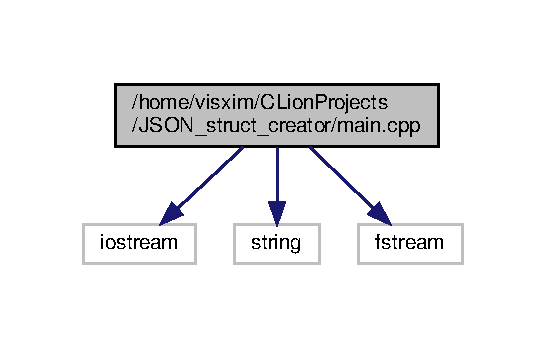
\includegraphics[width=262pt]{main_8cpp__incl}
\end{center}
\end{figure}
\subsection*{Functions}
\begin{DoxyCompactItemize}
\item 
void \hyperlink{main_8cpp_acf32301ca9b2f3977bf01ea7ed9ae437}{reset\+Values} ()
\begin{DoxyCompactList}\small\item\em resets the Values of the iterators \end{DoxyCompactList}\item 
string \hyperlink{main_8cpp_a5785c8b66c5d0c61fec7cc56414d98f6}{get\+\_\+string\+\_\+object} ()
\begin{DoxyCompactList}\small\item\em returns the next name from the object\+\_\+name array \end{DoxyCompactList}\item 
string \hyperlink{main_8cpp_aa408e57de9e02c4b7bf11ff322f21132}{get\+\_\+string\+\_\+value} ()
\begin{DoxyCompactList}\small\item\em returns the next value from the object\+\_\+value array \end{DoxyCompactList}\item 
uint8\+\_\+t \hyperlink{main_8cpp_a163606ea767ccd7121a44e2982c093a4}{create\+J\+S\+ON} (uint16\+\_\+t length)
\begin{DoxyCompactList}\small\item\em Function for creating the synthetic J\+S\+ON file with the given parameters. \end{DoxyCompactList}\item 
uint8\+\_\+t \hyperlink{main_8cpp_a086c4f879729a12dfd0582d3704bd220}{create\+Struct} (uint16\+\_\+t length)
\begin{DoxyCompactList}\small\item\em Function for creating the struct for the matching J\+S\+ON file. \end{DoxyCompactList}\item 
uint8\+\_\+t \hyperlink{main_8cpp_a8897326f34a0ca6223b3f848455360f2}{create\+Archive} (uint16\+\_\+t length)
\begin{DoxyCompactList}\small\item\em Function for creating the Archive for the matching J\+S\+ON file. \end{DoxyCompactList}\item 
uint8\+\_\+t \hyperlink{main_8cpp_a5b821fbe023849d9adcebaedf9700bc0}{create\+C\+RC} (uint16\+\_\+t length)
\begin{DoxyCompactList}\small\item\em Function for creating the C\+RC for the matching J\+S\+ON file. \end{DoxyCompactList}\item 
uint16\+\_\+t \hyperlink{main_8cpp_aaf49c506c666317381adec426d3712c1}{create\+Parse} (uint16\+\_\+t length)
\begin{DoxyCompactList}\small\item\em Function for creating the parse information for the matching J\+S\+ON file. \end{DoxyCompactList}\item 
int \hyperlink{main_8cpp_ae66f6b31b5ad750f1fe042a706a4e3d4}{main} ()
\begin{DoxyCompactList}\small\item\em main \end{DoxyCompactList}\end{DoxyCompactItemize}
\subsection*{Variables}
\begin{DoxyCompactItemize}
\item 
uint16\+\_\+t \hyperlink{main_8cpp_a3863543b943eca3e88c500a3aad3f071}{str\+\_\+obj\+\_\+itr} = 0
\item 
uint32\+\_\+t \hyperlink{main_8cpp_a1ad95c3b17361c0a66b8dc03580d882d}{str\+\_\+obj\+\_\+appe\+\_\+itr} = 0
\item 
uint16\+\_\+t \hyperlink{main_8cpp_abfa88bf10c2bc8484d5fb343a277e045}{str\+\_\+val\+\_\+itr} = 0
\item 
string \hyperlink{main_8cpp_a8a6b7e1f64a1fd2c6cdd116ac70e75bf}{object\+\_\+names} \mbox{[}10\mbox{]} = \{\char`\"{}name\char`\"{},\char`\"{}description\char`\"{},\char`\"{}mode\char`\"{},\char`\"{}version\char`\"{},\char`\"{}status\char`\"{},\char`\"{}path\char`\"{},\char`\"{}buffer\+\_\+size\char`\"{},\char`\"{}id\char`\"{},\char`\"{}number\char`\"{},\char`\"{}length\char`\"{}\}
\begin{DoxyCompactList}\small\item\em Definition of the String which will define the J\+S\+ON file structure. \end{DoxyCompactList}\item 
string \hyperlink{main_8cpp_ab650c940fe61806592cc4d468b7fc764}{object\+\_\+values} \mbox{[}10\mbox{]} = \{\char`\"{}J\+S\+O\+N\+\_\+creator\char`\"{},\char`\"{}dummy json\char`\"{},\char`\"{}shutdown\char`\"{},\char`\"{}V1.\+283\char`\"{},\char`\"{}running\char`\"{},\char`\"{}$\sim$/etc/tmp/process1/running\char`\"{},\char`\"{}2048\char`\"{},\char`\"{}1337\char`\"{},\char`\"{}1\char`\"{},\char`\"{}2309763\char`\"{}\}
\end{DoxyCompactItemize}


\subsection{Detailed Description}
main of the J\+S\+O\+N\+\_\+struct\+\_\+creator 

This project is for generating J\+S\+ON files and the neccessary code (struct, archive, C\+RC, parse) to run it. The size can be predefined by the number of cycles. A\+T\+T\+E\+N\+T\+I\+ON\+: These generated J\+S\+ON files are with the only purpose of simulating different sizes J\+S\+ON files, they depend on a repetitive algorithm. 

\subsection{Function Documentation}
\mbox{\Hypertarget{main_8cpp_a8897326f34a0ca6223b3f848455360f2}\label{main_8cpp_a8897326f34a0ca6223b3f848455360f2}} 
\index{main.\+cpp@{main.\+cpp}!create\+Archive@{create\+Archive}}
\index{create\+Archive@{create\+Archive}!main.\+cpp@{main.\+cpp}}
\subsubsection{\texorpdfstring{create\+Archive()}{createArchive()}}
{\footnotesize\ttfamily uint8\+\_\+t create\+Archive (\begin{DoxyParamCaption}\item[{uint16\+\_\+t}]{length }\end{DoxyParamCaption})}



Function for creating the Archive for the matching J\+S\+ON file. 

Here is the call graph for this function\+:
\nopagebreak
\begin{figure}[H]
\begin{center}
\leavevmode
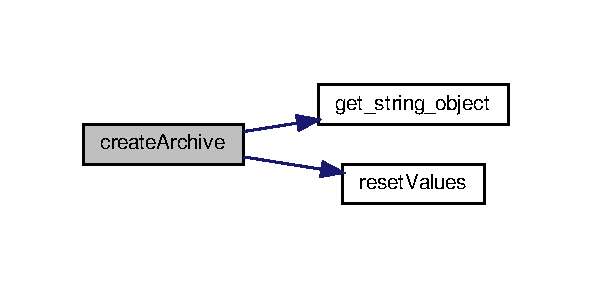
\includegraphics[width=284pt]{main_8cpp_a8897326f34a0ca6223b3f848455360f2_cgraph}
\end{center}
\end{figure}
\mbox{\Hypertarget{main_8cpp_a5b821fbe023849d9adcebaedf9700bc0}\label{main_8cpp_a5b821fbe023849d9adcebaedf9700bc0}} 
\index{main.\+cpp@{main.\+cpp}!create\+C\+RC@{create\+C\+RC}}
\index{create\+C\+RC@{create\+C\+RC}!main.\+cpp@{main.\+cpp}}
\subsubsection{\texorpdfstring{create\+C\+R\+C()}{createCRC()}}
{\footnotesize\ttfamily uint8\+\_\+t create\+C\+RC (\begin{DoxyParamCaption}\item[{uint16\+\_\+t}]{length }\end{DoxyParamCaption})}



Function for creating the C\+RC for the matching J\+S\+ON file. 

Here is the call graph for this function\+:
\nopagebreak
\begin{figure}[H]
\begin{center}
\leavevmode
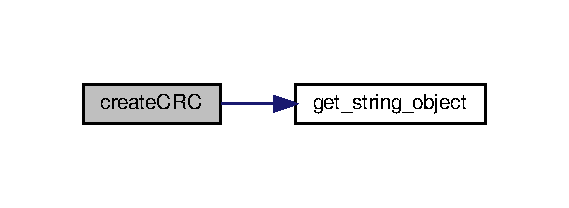
\includegraphics[width=273pt]{main_8cpp_a5b821fbe023849d9adcebaedf9700bc0_cgraph}
\end{center}
\end{figure}
\mbox{\Hypertarget{main_8cpp_a163606ea767ccd7121a44e2982c093a4}\label{main_8cpp_a163606ea767ccd7121a44e2982c093a4}} 
\index{main.\+cpp@{main.\+cpp}!create\+J\+S\+ON@{create\+J\+S\+ON}}
\index{create\+J\+S\+ON@{create\+J\+S\+ON}!main.\+cpp@{main.\+cpp}}
\subsubsection{\texorpdfstring{create\+J\+S\+O\+N()}{createJSON()}}
{\footnotesize\ttfamily uint8\+\_\+t create\+J\+S\+ON (\begin{DoxyParamCaption}\item[{uint16\+\_\+t}]{length }\end{DoxyParamCaption})}



Function for creating the synthetic J\+S\+ON file with the given parameters. 

Here is the call graph for this function\+:
\nopagebreak
\begin{figure}[H]
\begin{center}
\leavevmode
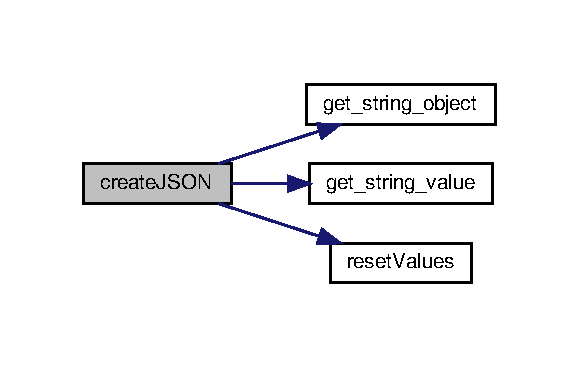
\includegraphics[width=278pt]{main_8cpp_a163606ea767ccd7121a44e2982c093a4_cgraph}
\end{center}
\end{figure}
\mbox{\Hypertarget{main_8cpp_aaf49c506c666317381adec426d3712c1}\label{main_8cpp_aaf49c506c666317381adec426d3712c1}} 
\index{main.\+cpp@{main.\+cpp}!create\+Parse@{create\+Parse}}
\index{create\+Parse@{create\+Parse}!main.\+cpp@{main.\+cpp}}
\subsubsection{\texorpdfstring{create\+Parse()}{createParse()}}
{\footnotesize\ttfamily uint16\+\_\+t create\+Parse (\begin{DoxyParamCaption}\item[{uint16\+\_\+t}]{length }\end{DoxyParamCaption})}



Function for creating the parse information for the matching J\+S\+ON file. 

Here is the call graph for this function\+:
\nopagebreak
\begin{figure}[H]
\begin{center}
\leavevmode
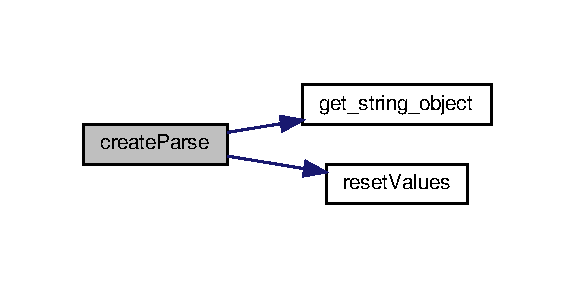
\includegraphics[width=276pt]{main_8cpp_aaf49c506c666317381adec426d3712c1_cgraph}
\end{center}
\end{figure}
\mbox{\Hypertarget{main_8cpp_a086c4f879729a12dfd0582d3704bd220}\label{main_8cpp_a086c4f879729a12dfd0582d3704bd220}} 
\index{main.\+cpp@{main.\+cpp}!create\+Struct@{create\+Struct}}
\index{create\+Struct@{create\+Struct}!main.\+cpp@{main.\+cpp}}
\subsubsection{\texorpdfstring{create\+Struct()}{createStruct()}}
{\footnotesize\ttfamily uint8\+\_\+t create\+Struct (\begin{DoxyParamCaption}\item[{uint16\+\_\+t}]{length }\end{DoxyParamCaption})}



Function for creating the struct for the matching J\+S\+ON file. 

Here is the call graph for this function\+:
\nopagebreak
\begin{figure}[H]
\begin{center}
\leavevmode
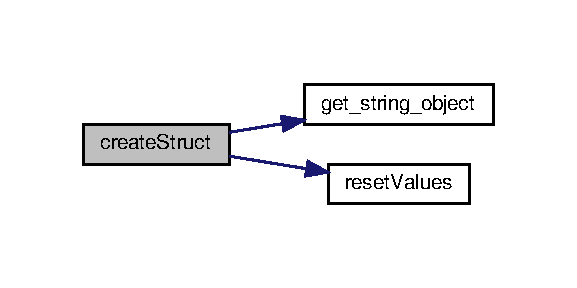
\includegraphics[width=277pt]{main_8cpp_a086c4f879729a12dfd0582d3704bd220_cgraph}
\end{center}
\end{figure}
\mbox{\Hypertarget{main_8cpp_a5785c8b66c5d0c61fec7cc56414d98f6}\label{main_8cpp_a5785c8b66c5d0c61fec7cc56414d98f6}} 
\index{main.\+cpp@{main.\+cpp}!get\+\_\+string\+\_\+object@{get\+\_\+string\+\_\+object}}
\index{get\+\_\+string\+\_\+object@{get\+\_\+string\+\_\+object}!main.\+cpp@{main.\+cpp}}
\subsubsection{\texorpdfstring{get\+\_\+string\+\_\+object()}{get\_string\_object()}}
{\footnotesize\ttfamily string get\+\_\+string\+\_\+object (\begin{DoxyParamCaption}{ }\end{DoxyParamCaption})}



returns the next name from the object\+\_\+name array 

\mbox{\Hypertarget{main_8cpp_aa408e57de9e02c4b7bf11ff322f21132}\label{main_8cpp_aa408e57de9e02c4b7bf11ff322f21132}} 
\index{main.\+cpp@{main.\+cpp}!get\+\_\+string\+\_\+value@{get\+\_\+string\+\_\+value}}
\index{get\+\_\+string\+\_\+value@{get\+\_\+string\+\_\+value}!main.\+cpp@{main.\+cpp}}
\subsubsection{\texorpdfstring{get\+\_\+string\+\_\+value()}{get\_string\_value()}}
{\footnotesize\ttfamily string get\+\_\+string\+\_\+value (\begin{DoxyParamCaption}{ }\end{DoxyParamCaption})}



returns the next value from the object\+\_\+value array 

\mbox{\Hypertarget{main_8cpp_ae66f6b31b5ad750f1fe042a706a4e3d4}\label{main_8cpp_ae66f6b31b5ad750f1fe042a706a4e3d4}} 
\index{main.\+cpp@{main.\+cpp}!main@{main}}
\index{main@{main}!main.\+cpp@{main.\+cpp}}
\subsubsection{\texorpdfstring{main()}{main()}}
{\footnotesize\ttfamily int main (\begin{DoxyParamCaption}{ }\end{DoxyParamCaption})}



main 

Declaration of the size of the J\+S\+ON file 100 $\sim$ 2,5kb

Creating all neccessary objects N\+O\+T\+I\+CE\+: J\+S\+ON file will be saved to Share\+Folder Here is the call graph for this function\+:
\nopagebreak
\begin{figure}[H]
\begin{center}
\leavevmode
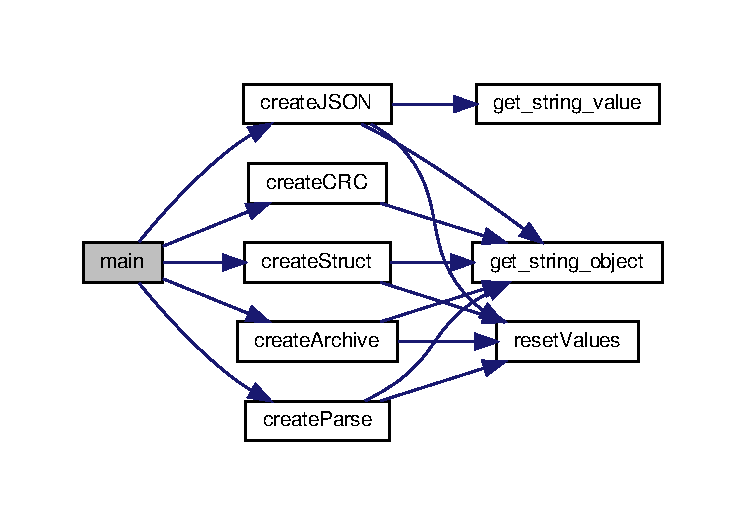
\includegraphics[width=350pt]{main_8cpp_ae66f6b31b5ad750f1fe042a706a4e3d4_cgraph}
\end{center}
\end{figure}
\mbox{\Hypertarget{main_8cpp_acf32301ca9b2f3977bf01ea7ed9ae437}\label{main_8cpp_acf32301ca9b2f3977bf01ea7ed9ae437}} 
\index{main.\+cpp@{main.\+cpp}!reset\+Values@{reset\+Values}}
\index{reset\+Values@{reset\+Values}!main.\+cpp@{main.\+cpp}}
\subsubsection{\texorpdfstring{reset\+Values()}{resetValues()}}
{\footnotesize\ttfamily void reset\+Values (\begin{DoxyParamCaption}{ }\end{DoxyParamCaption})}



resets the Values of the iterators 



\subsection{Variable Documentation}
\mbox{\Hypertarget{main_8cpp_a8a6b7e1f64a1fd2c6cdd116ac70e75bf}\label{main_8cpp_a8a6b7e1f64a1fd2c6cdd116ac70e75bf}} 
\index{main.\+cpp@{main.\+cpp}!object\+\_\+names@{object\+\_\+names}}
\index{object\+\_\+names@{object\+\_\+names}!main.\+cpp@{main.\+cpp}}
\subsubsection{\texorpdfstring{object\+\_\+names}{object\_names}}
{\footnotesize\ttfamily string object\+\_\+names\mbox{[}10\mbox{]} = \{\char`\"{}name\char`\"{},\char`\"{}description\char`\"{},\char`\"{}mode\char`\"{},\char`\"{}version\char`\"{},\char`\"{}status\char`\"{},\char`\"{}path\char`\"{},\char`\"{}buffer\+\_\+size\char`\"{},\char`\"{}id\char`\"{},\char`\"{}number\char`\"{},\char`\"{}length\char`\"{}\}}



Definition of the String which will define the J\+S\+ON file structure. 

\mbox{\Hypertarget{main_8cpp_ab650c940fe61806592cc4d468b7fc764}\label{main_8cpp_ab650c940fe61806592cc4d468b7fc764}} 
\index{main.\+cpp@{main.\+cpp}!object\+\_\+values@{object\+\_\+values}}
\index{object\+\_\+values@{object\+\_\+values}!main.\+cpp@{main.\+cpp}}
\subsubsection{\texorpdfstring{object\+\_\+values}{object\_values}}
{\footnotesize\ttfamily string object\+\_\+values\mbox{[}10\mbox{]} = \{\char`\"{}J\+S\+O\+N\+\_\+creator\char`\"{},\char`\"{}dummy json\char`\"{},\char`\"{}shutdown\char`\"{},\char`\"{}V1.\+283\char`\"{},\char`\"{}running\char`\"{},\char`\"{}$\sim$/etc/tmp/process1/running\char`\"{},\char`\"{}2048\char`\"{},\char`\"{}1337\char`\"{},\char`\"{}1\char`\"{},\char`\"{}2309763\char`\"{}\}}

\mbox{\Hypertarget{main_8cpp_a1ad95c3b17361c0a66b8dc03580d882d}\label{main_8cpp_a1ad95c3b17361c0a66b8dc03580d882d}} 
\index{main.\+cpp@{main.\+cpp}!str\+\_\+obj\+\_\+appe\+\_\+itr@{str\+\_\+obj\+\_\+appe\+\_\+itr}}
\index{str\+\_\+obj\+\_\+appe\+\_\+itr@{str\+\_\+obj\+\_\+appe\+\_\+itr}!main.\+cpp@{main.\+cpp}}
\subsubsection{\texorpdfstring{str\+\_\+obj\+\_\+appe\+\_\+itr}{str\_obj\_appe\_itr}}
{\footnotesize\ttfamily uint32\+\_\+t str\+\_\+obj\+\_\+appe\+\_\+itr = 0}

\mbox{\Hypertarget{main_8cpp_a3863543b943eca3e88c500a3aad3f071}\label{main_8cpp_a3863543b943eca3e88c500a3aad3f071}} 
\index{main.\+cpp@{main.\+cpp}!str\+\_\+obj\+\_\+itr@{str\+\_\+obj\+\_\+itr}}
\index{str\+\_\+obj\+\_\+itr@{str\+\_\+obj\+\_\+itr}!main.\+cpp@{main.\+cpp}}
\subsubsection{\texorpdfstring{str\+\_\+obj\+\_\+itr}{str\_obj\_itr}}
{\footnotesize\ttfamily uint16\+\_\+t str\+\_\+obj\+\_\+itr = 0}

\mbox{\Hypertarget{main_8cpp_abfa88bf10c2bc8484d5fb343a277e045}\label{main_8cpp_abfa88bf10c2bc8484d5fb343a277e045}} 
\index{main.\+cpp@{main.\+cpp}!str\+\_\+val\+\_\+itr@{str\+\_\+val\+\_\+itr}}
\index{str\+\_\+val\+\_\+itr@{str\+\_\+val\+\_\+itr}!main.\+cpp@{main.\+cpp}}
\subsubsection{\texorpdfstring{str\+\_\+val\+\_\+itr}{str\_val\_itr}}
{\footnotesize\ttfamily uint16\+\_\+t str\+\_\+val\+\_\+itr = 0}


%--- End generated contents ---

% Index
\backmatter
\newpage
\phantomsection
\clearemptydoublepage
\addcontentsline{toc}{chapter}{Index}
\printindex

\end{document}
